%%%
% set up document type
%%%
\documentclass[12pt]{article}

%%%
% declare all packages
%%%
\usepackage[left=25mm, top=20mm, right=25mm, bottom=30mm,nohead,nofoot]{geometry} 

\usepackage[T2A]{fontenc}
\usepackage[utf8]{inputenc}
\usepackage[english, russian]{babel}

\usepackage{graphics, graphicx}

\usepackage{url}
\usepackage{hyperref}

\usepackage{amssymb,latexsym} 
\usepackage{MnSymbol}
\usepackage{mathrsfs}

\usepackage[nottoc,numbib]{tocbibind}
\usepackage{float}
\usepackage{listings}
\usepackage{multirow}
\usepackage{hhline}

\usepackage{color,colortbl}

% \usepackage{verbatim}
%%%
% document settings
%%%
\setcounter{tocdepth}{4}
\graphicspath{ {./pic/} }

\renewcommand{\listoffigures}{\begingroup  % add number to list of graphics
\tocsection
\tocfile{\listfigurename}{lof}
\endgroup}
\renewcommand{\listoftables}{\begingroup  % add number to list of tables
\tocsection
\tocfile{\listtablename}{lot}
\endgroup}

%******************************************************************
%******************************************************************
\begin{document}

\begin{titlepage}
	\center
		Санкт-Петербургский Политехнический 
		университет \\ Петра Великого\\
		Институт прикладной математики и механики
		\\ \textbf{Кафедра «Прикладная математика»}

	\vfill ~
	\textbf{
		\\ \large ЛАБОРАТОРНАЯ РАБОТА №1
	}
	\\	на тему 
	\\ "Метод конечных разностей для ОДУ 2-го порядка"
	\\ по дисциплине
	\\ "Конечно-разностные и сеточные методы"

	\vfill ~

	Выполнил студент гр. \textbf{3630102/60101} \\
	\textbf{Лансков.Н.В.} \\ 

\vfill

{\large}	Санкт-Петербург
\\ 2019
\end{titlepage}

%%%
% Table of conetnts 
%%%

\tableofcontents 
\newpage
\listoffigures
\newpage
\listoftables
\newpage

%%%
% Text
%%%
\section{Постановка задачи}

Рассмотрим задачу :

$$
\begin{cases}
-\dfrac{d^2u}{dx^2} + e^x\dfrac{du}{dx} + u(cos^2(x) + 1) = f(x), & x \in [0.5;2] \\ \\
\dfrac{du}{dx}(0.5) + u(0.5) = e^{0.5}sin(e^{0.5}) - cos(e^{0.5}) \\ \\
\dfrac{du}{dx}(2) + u(2) = e^2cos(e^2) + sin(e^2)
\end{cases}
$$

Где:
$$
f(x) = -e^xcos(e^x) + e^{2x}sin(e^x) + e^{2x}cos(e^x) + sin(e^x)(sin^2(x) + 1)
$$

Точное решение задачи : $u(x) = sin(e^x)$ 
\section{Разностные схемы}
\subsection{Разностная схема $O(h^2)$}
Введём регулярную сетку:
$$
\Omega_h(x) = \{x_i | x_i = 0,5 + ih, i = \overline{0, M}, h = \dfrac{1}{M}\}
$$

Выбор шага h будет осуществляться несколько раз для сравнения полученных результатов при различных шагах.
Выберем следующий шаблон аппроксимации:
$$
\omega_h(x_i) = \{ x_{i-1}; x_i; x_{i + 1}\}
$$

при выборе данного шаблона для аппроксимации первой и второй производной  мы получим требуемую погрешность . Для такого шаблона ранее были выведены аппроксимации первой и второй производных, а именно:

$$
u_{\dot{x}} = \dfrac{u_{i + 1} - u_{i - 1}}{2h}
$$

$$
u_{\overline{x}x} = \dfrac{u_{i + 1} -2u_i+ u_{i - 1}}{h^2}
$$

Тогда можем переписать исходную задачу, используя сеточную функцию v(x) – приближение к u(x) следующим образом:

$$
\begin{cases}
-\dfrac{v_{i+1} - 2v_i + v_{i-1}}{h^2} + e^x\dfrac{v_{i+1} - v_{i-1}}{2h} + v_i(sin^2(x) + 1) = f_i^* \\
\\
- \dfrac{-3v_0 + 4v_1 - v_2}{2h} + v_0 = e^{0.5}sin(e^{0.5}) - cos(e^{0.5}) \\
\\
\dfrac{3v_M - 4v_{M-1} + v_{M-2}}{2h} + v_M = e^2cos(e^2) + sin(e^2)
\end{cases}
$$

Стоит обратить внимание на аппроксимацию на краях отрезка, для них используется другие шаблоны аппроксимации:
$$
\omega_h(x_0) = \{ x_{0}; x_{1}; x_{2}\}
$$

$$
\omega_h(x_M) = \{ x_M; x_{M - 1}; x_{M - 2}\}
$$

Ранее доказано, что выбор данных шаблонов аппроксимации обеспечит нам общую погрешность разностной схемы как 
$O(h^2)$

Тогда, перегруппировав слагаемые, получим СЛАУ, которую будем решать методом прогонки, у искомой СЛАУ получим трехдиагональную матрицу коэффициентов.

$$
\begin{cases}
v_{i-1}(-\dfrac{1}{h^2} - \dfrac{e^{x_i}}{2h}) + v_i(\dfrac{2}{h^2} + sin^2(x_i) + 1) + v_{i + 1}(-\dfrac{1}{h^2} + \dfrac{e^{x_i}}{2h}) = f_i^*\\
\\
v_o(\dfrac{3}{2h}  +1) + v_1(-\dfrac{2}{h}) + v_2(\dfrac{1}{2h}) = e^{0.5}sin(e^{0.5}) - cos(e^{0.5})\\
\\
v_{M-2}(\dfrac{1}{2h}) + v_{M-1}(-\dfrac{2}{h})  +v_M(\dfrac{3}{2h} + 1) = e^2cos(e^2) + sin(e^2)
\end{cases}
$$

В итоге получена матрица коэффициентов:

$$
\begin{pmatrix}
	\dfrac{3}{2h}  +1 & -\dfrac{2}{h} &  \dfrac{1}{2h} & 0 & ... \\
	\\
	-\dfrac{1}{h^2} - \dfrac{e^{x_2}}{2h} & \dfrac{2}{h^2} + sin^2(x_2) + 1 & -\dfrac{1}{h^2} + \dfrac{e^{x_2}}{2h} & 0 & ... \\
	\\
	0 & -\dfrac{1}{h^2} - \dfrac{e^{x_3}}{2h} & \dfrac{2}{h^2} + sin^2(x_3) + 1 & -\dfrac{1}{h^2} + \dfrac{e^{x_3}}{2h} & ... \\
	... & ... & ... & ... & ... \\
	\\
	... & 0 & -\dfrac{1}{h^2} - \dfrac{e^{x_{M-1}}}{2h} & \dfrac{2}{h^2} + sin^2(x_{M-1}) + 1 & -\dfrac{1}{h^2} + \dfrac{e^{x_{M-1}}}{2h} \\
	\\
	... & 0 & \dfrac{1}{2h} & -\dfrac{2}{h} &\dfrac{3}{2h} + 1 \\
\end{pmatrix}
$$

С правой частью из $sin(1) - cos(1), e^2cos(e^2) + sin(e^2)$ и  $f_i^*$ для $i = \overline{2, M-1}$. Для того, чтобы решить данную СЛАУ методом прогонки и получить искомый результат, необходимо привести матрицу к трехдиагональному виду. Домножаем вторую строку на выражение $ - \dfrac{\dfrac{1}{2h}}{-\dfrac{1}{h^2} + \dfrac{e^{x_2}}{2h}} $ (с учётом правой части!) и прибавляем к первой. Аналогичным образом поступаем для "правки" последней строки. В результате получается трёхдиагональная матрица, которая уже непосредственно используется в методе прогонки:


$$
\begin{pmatrix}
	(\dfrac{3}{2h}  +1)( - \dfrac{\dfrac{1}{2h}}{-\dfrac{1}{h^2} + \dfrac{e^{x_2}}{2h}})& 
	(-\dfrac{2}{h})( - \dfrac{\dfrac{1}{2h}}{-\dfrac{1}{h^2} + \dfrac{e^{x_2}}{2h}}) &  0 & 0 & ... \\
	\\
	-\dfrac{1}{h^2} - \dfrac{e^{x_2}}{2h} & \dfrac{2}{h^2} + sin^2(x_2) + 1 & ... & 0 & ... \\
	\\
	0 & -\dfrac{1}{h^2} - \dfrac{e^{x_3}}{2h} & ... & -\dfrac{1}{h^2} + \dfrac{e^{x_3}}{2h} & ... \\
	... & ... & ... & ... & ... \\
	\\
	... & 0 & ... & \dfrac{2}{h^2} + sin^2(x_{M-1}) + 1 & -\dfrac{1}{h^2} + \dfrac{e^{x_{M-1}}}{2h} \\
	\\
	... & 0 & 0 & (-\dfrac{2}{h})( - \dfrac{\dfrac{1}{2h}}{-\dfrac{1}{h^2} - \dfrac{e^{x_{M-1}}}{2h}}) &
	(\dfrac{3}{2h} + 1)( - \dfrac{\dfrac{1}{2h}}{-\dfrac{1}{h^2} - \dfrac{e^{x_{M-1}}}{2h}}) \\
\end{pmatrix}
$$

\subsection{Разностная схема $O(h)$}

Аналогично предыдущему пункту, выберем сетку:
Для этого введем регулярную сетку:

$$
\Omega_h(x) = \{x_i | x_i = ih, i = \overline{0, M}, h = \dfrac{1}{M}\}
$$

причем выбор шага h будет осуществляться несколько раз для сравнения полученных результатов при различных шагах.
Для второй производной выберем использованный ранее шаблон аппроксимации, для первой производной шаблон апроксимации будет иметь вид:
$$
\omega_h(x_i) = \{ x_{i}; x_{i + 1}\}
$$
Тогда :
$$
u_x = \dfrac{u_{i + 1} - u_{i}}{h}
$$

Проводя аналогичные предыдущему пункту рассуждения, перейдем от исходной задачи к разностной схеме. В этом случае, так как нам требуется точность всего лишь O(h), то условия на границах можно аппроксимировать чуть более простой разностной схемой с тем же шаблоном, что используется для аппроксимации первой производной.

$$
\begin{cases}
- \dfrac{v_{i+1} - 2v_i + v_{i - 1}}{h^2} + e^{x_i}\dfrac{v_{i+1} - v_i}{h} + v_i(sin^2(x_i) + 1) = f_i^* \\
\\
- \dfrac{v_1 - v_0}{h} + v_0 = e^{0.5}sin(e^{0.5}) - cos(e^{0.5}) \\
\\
\dfrac{v_M - v_{M-1}}{h} + v_M = e^2cos(e^2) + sin(e^2)
\end{cases}
$$


Иными словами, сразу получаем трёхдиагональную матрицу. Решаем методом прогонки.

$$
\begin{pmatrix}
	\dfrac{1}{h} + 1& -\dfrac{1}{h} &  0 & 0 & ... \\
	\\
	-\dfrac{1}{h^2}  & \dfrac{2}{h^2} - \dfrac{e^{x_2}}{h} + sin^2(x_2) + 1 & -\dfrac{1}{h^2} + \dfrac{e^{x_2}}{h} & 0 & ... \\
	\\
	0 & -\dfrac{1}{h^2} & \dfrac{2}{h^2} - \dfrac{e^{x_3}}{h} + sin^2(x_3) + 1 &
	 -\dfrac{1}{h^2} + \dfrac{e^{x_3}}{h} & ... \\
	... & ... & ... & ... & ... \\
	\\
	... & 0 & \dfrac{-1}{h^2} & \dfrac{2}{h^2} - \dfrac{e^{x_3}}{h} + sin^2(x_3) + 1 &
	 -\dfrac{1}{h^2} + \dfrac{e^{x_{M-1}}}{h} \\
	\\
	... & 0 & 0 & -\dfrac{1}{h} & \dfrac{1}{h} + 1\\
\end{pmatrix}
$$
\newpage
\section{Результаты}
Для определения погрешности найдем следующую норму:
$$
||z_h|| = || u_h - v_h ||
$$
Норму будем вычислять по формуле:
$$
||x|| = \sqrt{h\sum\limits_{i=1}^M x_i^2}
$$

Будем смотреть, как изменится это значение в зависимости от размера шага h. Также построим зависимость  от  и исследуем угловой коэффициент прямой, отражающей эту зависимость. Составим таблицу, отражающую полученные зависимости:

\subsection{Разностная схема $O(h^2)$}

\begin{table}[H]
\caption{Зависимость погрешности от числа узлов}
\begin{center}
\begin{tabular}{|c|c|c|}
\hline
\textit{Число узлов} &$ h$ & $||z_h||$  \\
\hline
20 & 0.078947 & 0.021510 \\
\hline
40 & 0.038462 & 0.0051808 \\
\hline
80 & 0.018987 & 0.0012575 \\
\hline
160 & 0.0094340 & 3.0894e-04 \\
\hline
320 & 0.0047022 & 7.6522e-05 \\
\hline
640 & 0.0023474 & 1.9039e-05 \\
\hline
1280 & 0.0011728 & 4.7483e-06 \\
\hline
2560 & 5.8617e-04 & 1.1856e-06 \\
\hline
5120 & 2.9303e-04 & 2.9623e-07 \\
\hline
10240 & 1.4650e-04 & 7.4034e-08 \\
\hline
20480 & 7.3246e-05 & 1.8517e-08 \\
\hline
40960 & 3.6622e-05 & 4.6819e-09 \\
\hline
81920 & 1.8311e-05 & 1.5348e-09 \\
\hline
163840 & 9.1553e-06 & 2.6090e-09 \\
\hline

\end{tabular}
\end{center}
\end{table}


Заметно, что при уменьшении шага погрешность приближенного решения уменьшается, но лишь до определенного значения числа h. Оказывается, оптимальное (в плане точности) число узлов в данной задаче и при данной схеме – около 80000, дальше погрешность начинает быть сравнима с погрешностью округления.

\begin{figure}
\begin{center}
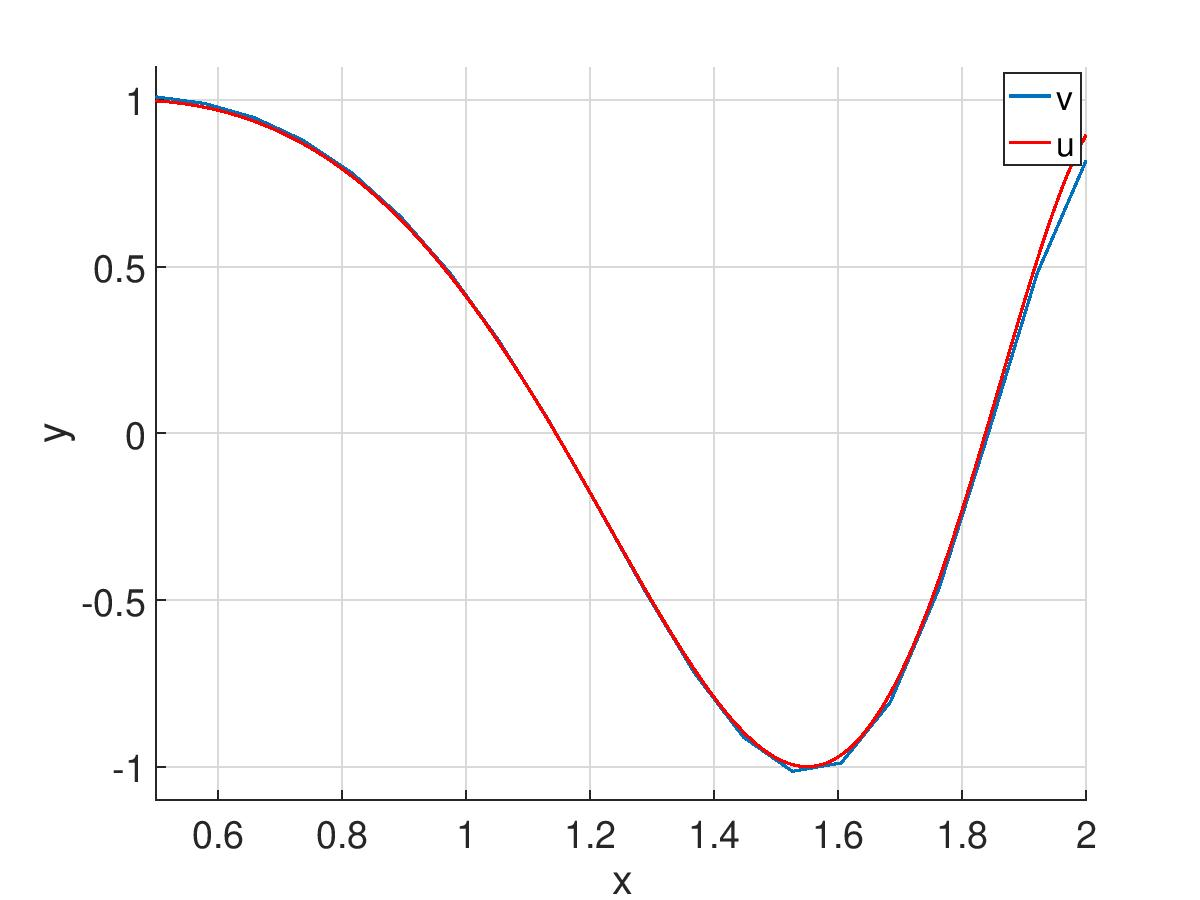
\includegraphics[scale = 0.5]{h2_20.jpg} 
\end{center}
\caption{$O(h^2), n = 20$ }
\end{figure}

\begin{figure}
\begin{center}
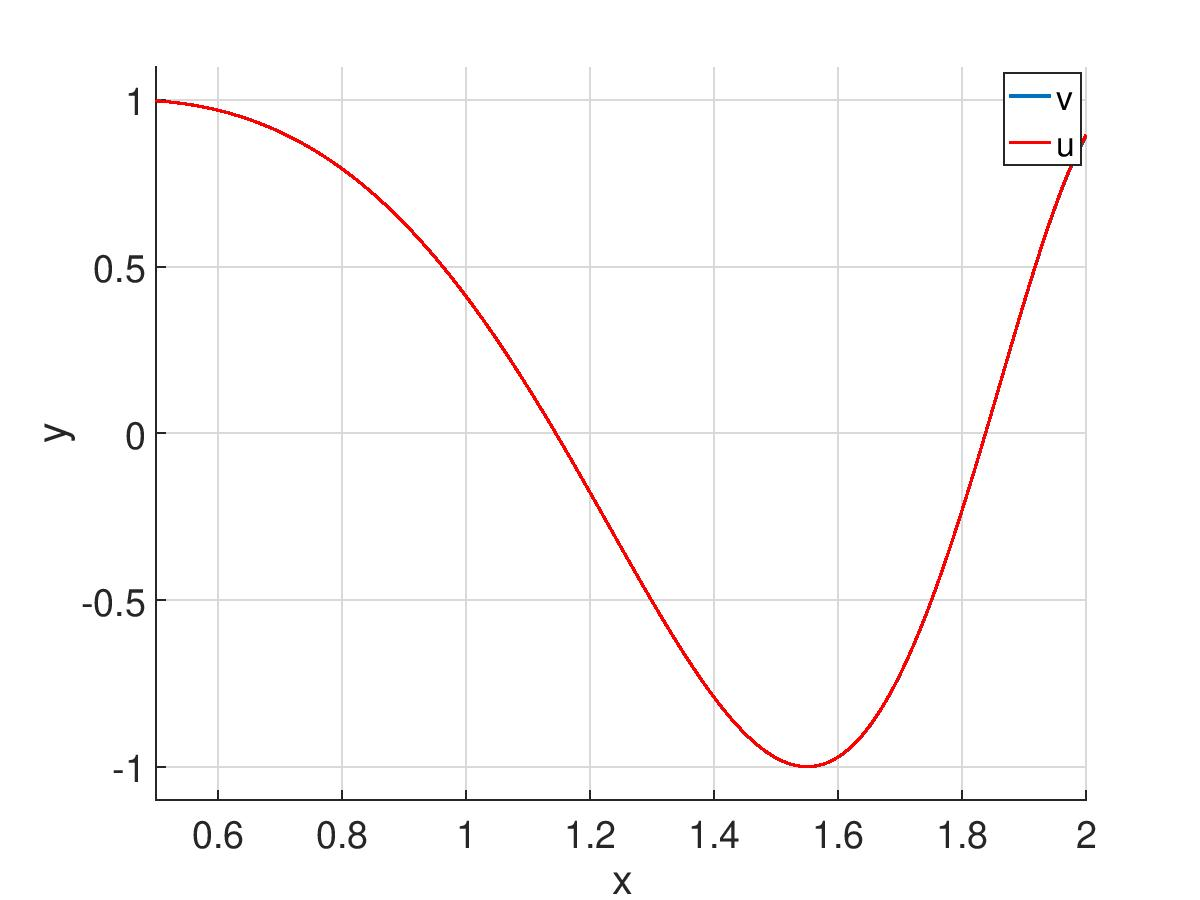
\includegraphics[scale = 0.5]{h2_100.jpg} 
\end{center}
\caption{$O(h^2), n = 100$ }
\end{figure}

\subsection{Разностная схема $O(h)$}

\begin{table}[H]
\caption{Зависимость погрешности от числа узлов}
\begin{center}
\begin{tabular}{|c|c|c|}
\hline
\textit{Число узлов} &$ h$ & $||z_h||$  \\
\hline
20 & 0.078947 & 0.10925 \\
\hline
40 & 0.038462 & 0.053382 \\
\hline
80 & 0.018987 & 0.026531 \\
\hline
160 & 0.0094340 & 0.013241\\
\hline
320 & 0.0047022 & 0.0066162 \\
\hline
640 & 0.0023474 & 0.0033072 \\
\hline
1280 & 0.0011728 &  0.0016534\\
\hline
2560 & 5.8617e-04 & 8.2667e-04 \\
\hline
5120 & 2.9303e-04 & 4.1333e-04 \\
\hline
10240 & 1.4650e-04 & 2.0666e-04 \\
\hline
20480 & 7.3246e-05 & 1.0333e-04 \\
\hline
40960 & 3.6622e-05 & 5.1665e-05 \\
\hline
81920 & 1.8311e-05 & 2.5833e-05 \\
\hline
163840 & 9.1553e-06 & 1.2916e-05 \\
\hline
327680 & 4.5777e-06 & 6.4803e-06 \\
\hline
655360 & 2.2888e-06 & 3.2328e-06 \\
\hline
1310720 & 1.1444e-06 & 1.5893e-06 \\
\hline
2621440 & 5.7220e-07 & 1.0271e-06 \\
\hline
5242880 & 2.8610e-07 & 7.6183e-06 \\
\hline
\end{tabular}
\end{center}
\end{table}

Также, как и в предыдущем случае, заметно, что с какого-то момента точность вычислений перестает повышаться, даже напротив – начинает падать. В данном случае погрешность начинает расти, когда число узлов доходит примерно до 5000000, что намного больше аналогичного значения у предыдущего способа аппроксимации.

\begin{figure}
\begin{center}
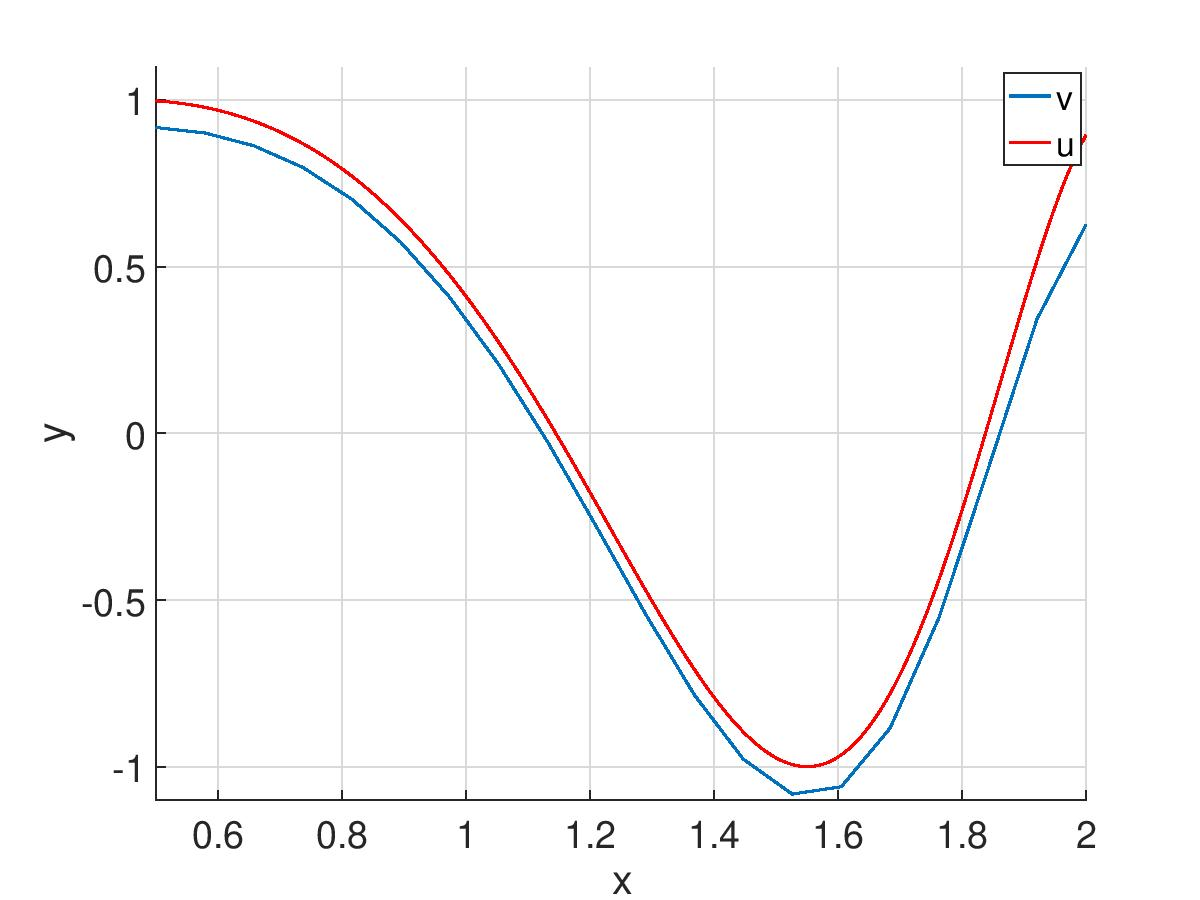
\includegraphics[scale = 0.5]{h1_20.jpg} 
\end{center}
\caption{$O(h), n = 20$ }
\end{figure}

\begin{figure}
\begin{center}
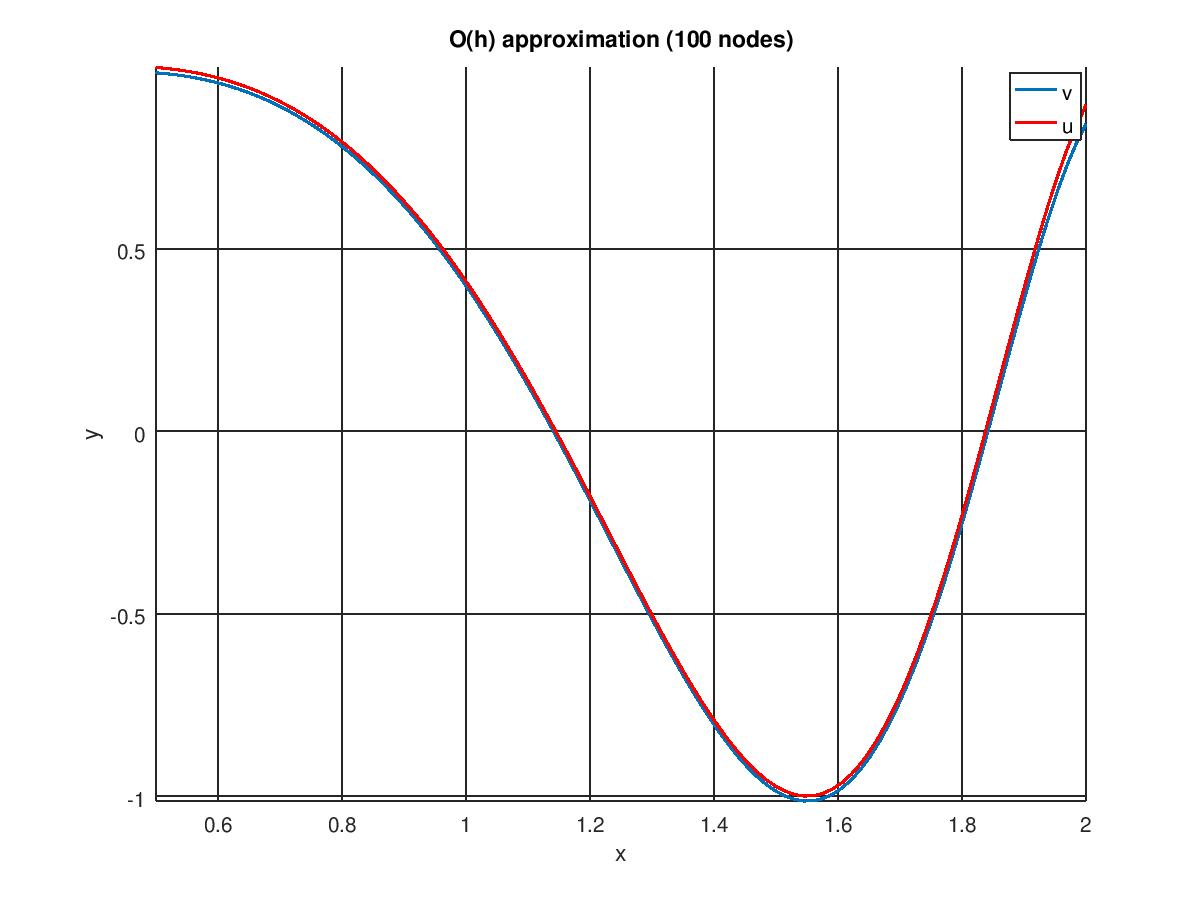
\includegraphics[scale = 0.5]{h1_100.jpg} 
\end{center}
\caption{$O(h), n = 100$}
\end{figure}


\pagebreak

\subsection{Зависимости погрешности от шага}

\begin{table}[H]
\caption{Зависимость погрешности от шага}
\begin{center}
\begin{tabular}{|c|c|c|}
\hline
$h$ & $||z_h||$ & $k$ \\
\hline
0.0011728 & 4.7483e-06 & 2 \\
\hline
5.8617e-04 & 1.1856e-06 & 2 \\
\hline
2.9303e-04 & 2.9623e-07 & 2 \\
\hline
7.3246e-05 & 7.4034e-08 & 2 \\
\hline
3.6622e-05 & 1.8517e-08 & 2 \\
\hline
1.8311e-05 & 4.6819e-09 & 2 \\
\hline
9.1553e-06 & 1.5348e-09 & 2 \\
\hline
4.5777e-06 & 2.6090e-09 & 2 \\
\hline
\hline
0.0011728 & 0.0016534 & 1 \\
\hline
5.8617e-04 & 8.2667e-04 & 1 \\
\hline
2.9303e-04 & 4.1333e-04 & 1 \\
\hline
7.3246e-05 & 2.0666e-04 & 1 \\
\hline
3.6622e-05 & 1.0333e-04 & 1 \\
\hline
1.8311e-05 & 5.1665e-05 & 1 \\
\hline
9.1553e-06 & 2.5833e-05 & 1 \\
\hline
4.5777e-06 & 1.2916e-05 & 1 \\
\hline
\end{tabular}
\end{center}
\end{table}

Построим графики зависимостей логарифма нормы разности точного и приближенного решения от логарифма шага. Рядом изобразим прямые с угловыми коэффициентами 1 и 2 соответственно для схем O(h) и O($h^2$). Из графиков видно, что логарифмические прямые имеют угловой коэффициент наклона, соответствующий порядку точности схемы, что согласуется с теорией. Также видно явление, при котором начиная с определённого момента мы достигли погрешности округления, и логарифмическая "прямая" перестаёт быть прямой.

\newpage

\begin{figure}
\begin{center}
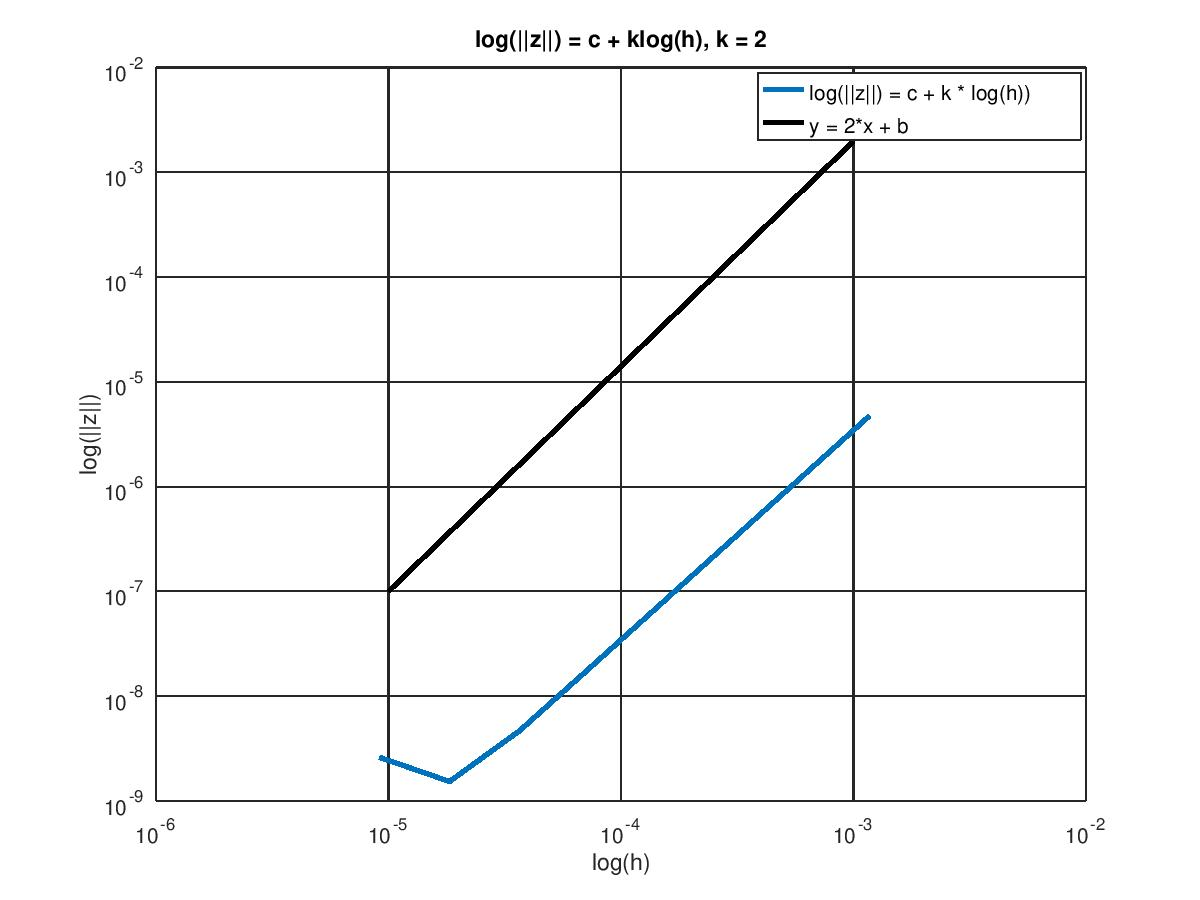
\includegraphics[scale = 0.4]{loglog2.jpg} 
\end{center}
\caption{$O(h^2)$}
\end{figure}

\begin{figure}
\begin{center}
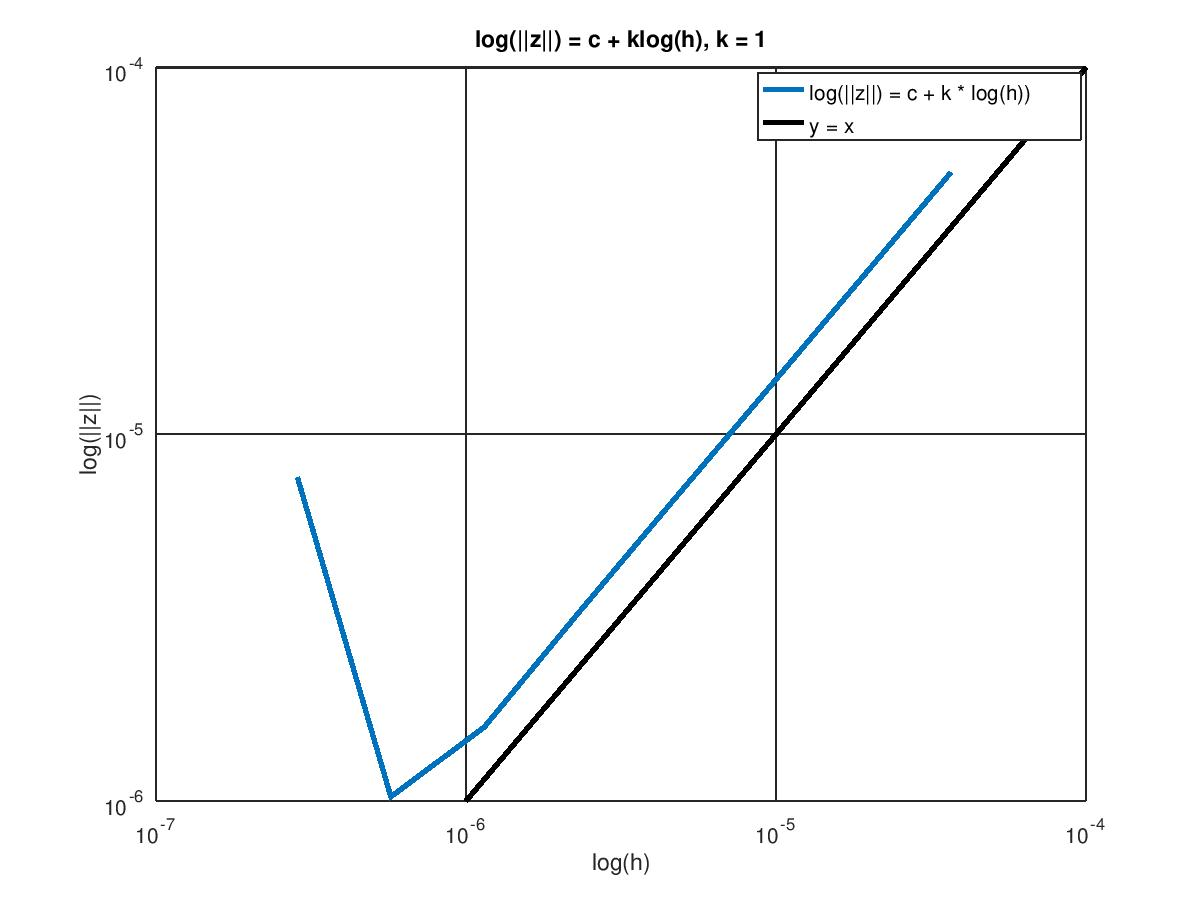
\includegraphics[scale = 0.4]{loglog1.jpg} 
\end{center}
\caption{$O(h)$}
\end{figure}

\section{Выводы}

В результате проведенной работы для исходной задачи были построены две разностные схемы с разным порядком аппроксимации. Были получены результаты, подтверждающие предположения о величине погрешности для разных схем. Также были получены свидетельства существования эффекта ухудшения погрешности при дроблении шага аппроксимации сверх определенного. Была показана разница в числе узлов, необходимых для достижения заданной погрешности для двух разностных схем и подтверждена большая эффективность схемы с более высоким порядком точности. Наконец, были получены зависимости величины погрешности от шага для разностных схем и наглядно показана разница между порядками аппроксимации в такой зависимости.

\end{document}

